\documentclass{article}
\usepackage[utf8]{inputenc}
\usepackage{graphicx}
\usepackage{makeidx}
\usepackage{geometry}
\usepackage{float}
\usepackage{indentfirst}

\renewcommand{\contentsname}{Índice}
\geometry{a4paper,total = {150mm,250mm},left = {30mm}, top = {30mm}}
\makeindex
\graphicspath{ {./imagens/} }
\begin{document}
\begin{capa}
	\begin{center}
	\vspace*{1.0cm}
	\huge{Universidade do Minho}\\
	[1.0cm]
	
\includegraphics{logo.jpg}\\
	[1.5cm]
	\huge{\textbf{Redes de Computadores}}\\
	[0.5cm]
	\textsc{RC-TP4}\\
	\textsc{\normalsize{Mestrado Integrado em Engenharia Informática}}\\
	\textsc{\normalsize{3º Ano}}\\
	\textsc{\normalsize{Grupo 61}}\\
	[12.0cm]
	\end{center}
	\begin{flushleft}
	\textsc{Renato André Araújo Azevedo \textbf{\hspace*{130pt} A89547}}\\
	\textsc{Gonçalo Costa de Almeida \textbf{\hspace*{151pt} A88292}}\\
	\textsc{Maria Sofia Martinho Gonçalves Jordão Marques \textbf{\hspace*{30pt} A87963}}\\
	\end{flushleft}
\end{capa}

\newpage
\tableofcontents
\newpage

\section{Introdução}
	No âmbito da cadeira de Redes Computadores foi-nos proposta a elaboração de um trabalho
	que terá como principal objetivo  o estudo das redes sem fios e as suas principais vertentes,
	nomeadamente: o estudo do protocolo IEEE 802.11, onde exploramos o formato das tramas,
	o endereçamento dos componentes envolvidos na comunicação sem fios,
	os tipos de tramas, bem como o modo de operação do protocolo.\par
	Esperamos, com este trabalho, atingir os objetivos definidos pelo docente. \\

\section{Acesso Rádio}
\subsection{Ex1}
\textbf{Identifique em que frequência do espectro está a operar a rede sem fios, e o canal que corresponde essa frequência.}\\\par
O espectro está a operar na frequencia 2467MHz (\textit{Frequency: 12}), e o canal correspondente é o 12 (\textit{Channel: 12}). 
\begin{figure}[h]
	\centering
	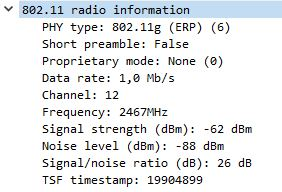
\includegraphics[scale = 0.8]{ex-1.JPG}
	\caption{Informação do canal}
\end{figure}

\subsection{Ex2}
\textbf{Identifique a versão da norma IEEE 802.11 que está a ser usada.}\\\par
A versão da norma IEEE 802.11 utilizada é 802.11g, como podemos observar pelo campo \textit{PHY type}.

\subsection{Ex3}
\textbf{Qual o débito a que foi enviada a trama escolhida? Será que esse débito corresponde ao débito máximo a que a interface WiFi pode operar? Justifique.}\\\par
O débito a que a trama foi enviada foi de 1 Mb/s, como podemos observar pela imagem no campo \textit{Data rate}.
No entanto esse débito não correpsonde ao débito máximo a que a interface pode operar, uma vez que o protocolo 802.11g permite débitos até 54 Mb/s.

\section{Scanning Passivo e Scanning Ativo}
\subsection{Ex4}
\textbf{Selecione uma trama beacon (e.g., trama 10XX). Esta trama pertence a que tipo de tramas 802.11? Indique o valor dos seus identificadores de tipo e de subtipo. Em que parte concreta do cabeçalho da trama estão especificados (ver anexo)?
}\\\par
Selecionando a trama 1061 podemos verificar que esta correponde a uma trama do tipo 802.11, sendo o seu tipo e subtipo identificados no campo frame control, como podemos retirar da imagem a baixo.\\
\begin{center}
Type: Management frame (0)\\
Subtype: 8
\end{center}
\begin{figure}[h]
	\centering
	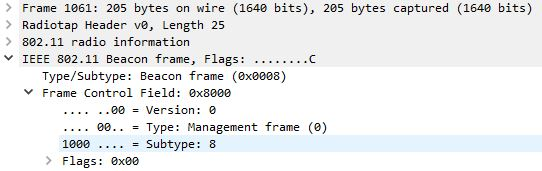
\includegraphics[scale = 0.8]{ex-4.JPG}
	\caption{Frame control trama 1061}
\end{figure}

\subsection{Ex5}
\textbf{Para a trama acima, identifique todos os endereços MAC em uso. Que conclui quanto à sua origem e destino?}\\\par
Os endereços MAP identidicados na trama são ff:ff:ff:ff:ff:ff, que corresponde ao endreço MAC do destino, e o endereço bc:14:01:af:b1:99 que corresponde simultaneamente ao AP que transmitiu a trama a trama e ao router à qual o AP está ligado, podendo concluir que o router e o AP estão juntos. Desta forma, podemos concluir que a origem da trama foi no AP e o destino é toda a rede, o que faz sentido, já que se trata de uma trama beacon.
\begin{figure}[h]
	\centering
	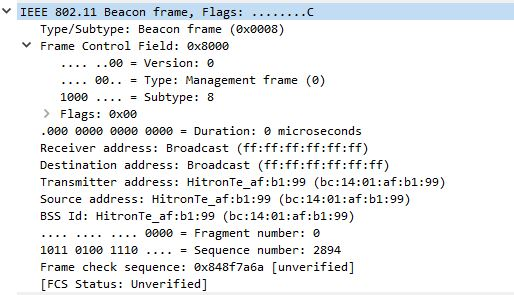
\includegraphics[scale = 0.7]{ex-5.JPG}
	\caption{Endereços da trama}
\end{figure}

\subsection{Ex6}
\textbf{Uma trama beacon anuncia que o AP pode suportar vários débitos de base, assim como vários débitos adicionais (extended supported rates). Indique quais são esses débitos?}\\\par
O AP consegue suportar vários débitos de base de 1 MB até 54 MB, além de débitos adicionais entre 6 MB até 48 MB, como podemos observar na seguinte imagem.
\begin{figure}[h]
	\centering
	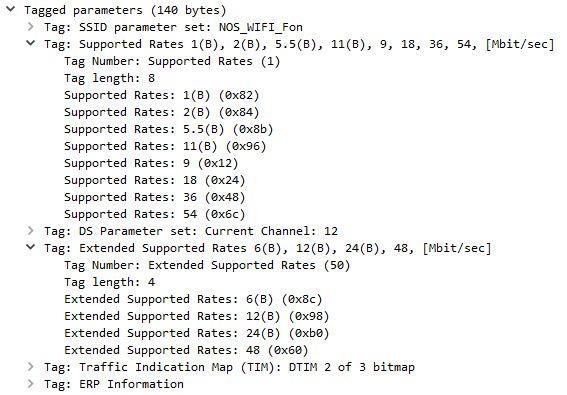
\includegraphics[scale = 0.6]{ex-6.JPG}
	\caption{Debitos}
\end{figure}

\subsection{Ex7}
\textbf{Qual o intervalo de tempo previsto entre tramas beacon consecutivas? (nota: este valor é anunciado na própria trama beacon). Na prática, a periodicidade de tramas beacon provenientes do mesmo AP é verificada? Tente explicar porquê.}\\\par
O intervalo de tempo entre tramas consecutivas é vísivel no campo Beacon Interval ao qual corresponde o tempo 0,102400 [Seconds], enquanto que o intervalo verificado é de 0.102275.
Tendo isso em conta é possivel verificar que o tempo entre essas tramas consecutivas de facto não se verifica. Isto pode acontecer por alguma falta de precisão de um AP que pode estar a enviar a trama mais cedo do q o suposto.

\begin{figure}[h]
	\centering
	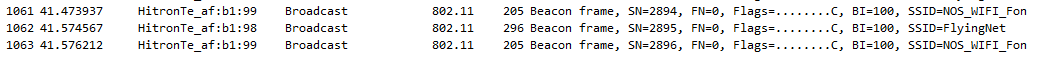
\includegraphics[scale = 0.5]{ex7TP4.png}
	\caption{Intervalo de tempo verificado}
\end{figure}

\begin{figure}[h]
	\centering
	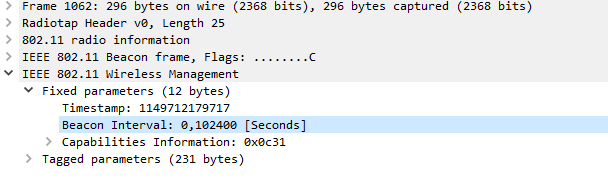
\includegraphics[scale = 0.8]{ex7.1.png}
	\caption{Intervalo de tempo da trama beacon}
\end{figure}

\subsection{Ex8}
\textbf{Identifique e liste os SSIDs dos APs que estão a operar na vizinhança da STA de captura? Explicite o modo como obteve essa informação (por exemplo, se usou algum filtro para o efeito).}\\\par
Como vimos na pergunta 4, os \texit{Beacon} tem o campo \textit{Subtype} com o valor 0x08. Desta forma, podemos criar um filtro que escolha todas as tramas cujo campo tenha este valor, o que fica wlan.fc.type\_subtype == 0x8. Desta forma, podemos observar que os SSIDs dos APs que estão a operar na vizinhança da STA de captura são o NOS\_WIFI\_Fon e o FlyingNet.
\begin{figure}[h]
	\centering
	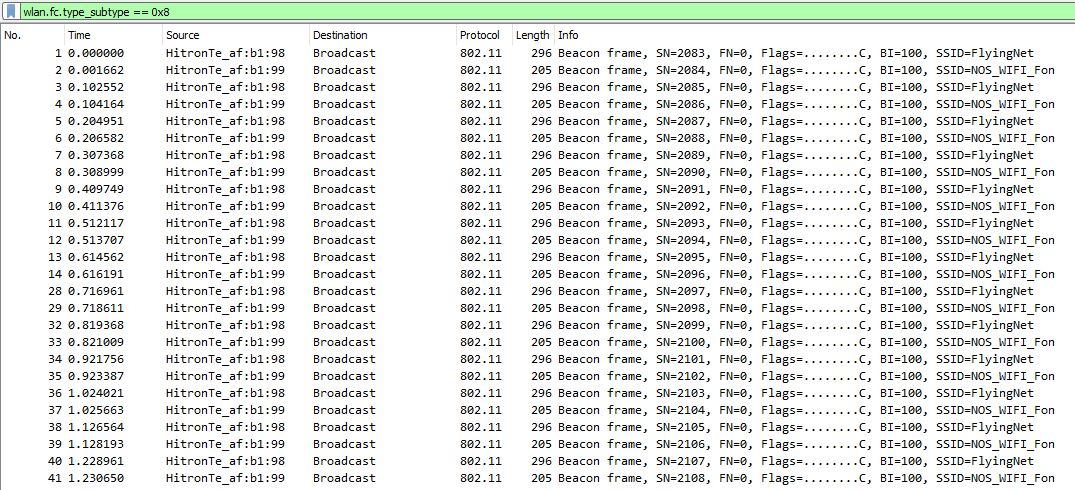
\includegraphics[scale = 0.5]{ex-8.JPG}
	\caption{Pontos de acesso na vizinhança}
\end{figure}

\subsection{Ex9}
\textbf{Verifique se está a ser usado o método de deteção de erros (CRC). Justifique.}\\\par
O método de detenção de erro está a ser utilizado conforme podemos ver no exemplo.
As redes sem fios estão sujeitas a taxas de erros muito mais intensas e variáveis do que as redes cabladas, devido a diversos factores, como ruído, interferência de outras fontes, obstrução do sinal, etc. Assim sendo é necessário a utilização da detenção de erros. 
\begin{figure}[h]
	\centering
	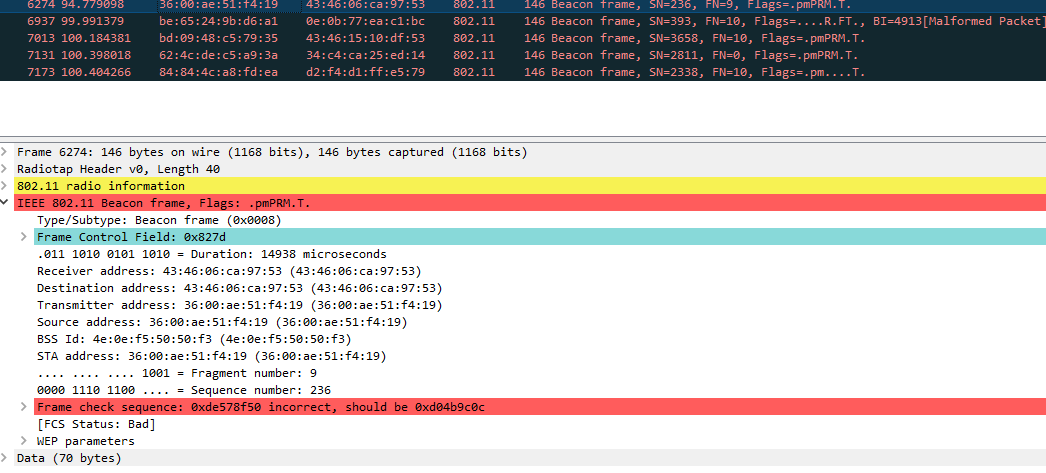
\includegraphics[scale = 0.5]{ex9TP4.PNG}
	\caption{Trama com erros}
\end{figure}

\subsection{Ex10}
\textbf{Estabeleça um filtro Wireshark apropriado que lhe permita visualizar todas as tramas probing request ou probing response, simultaneamente.}\\\par
Uma vez que no campo \texit{Subtype}, o \textit{probing request} tem associado o valor 0x4 e o \textit{probing response} tem associado o valor 0x5, então podemos aplicar o filtro "wlan.fc.type\_subtype in {0x4 0x5}", que vai filtrar todas as tramas cujo valor no campo \textit{Subtype} seja 0x4 ou 0x5.

\newpage
\subsection{Ex11}
\textbf{Identifique um probing request para o qual tenha havido um probing response. Face ao endereçamento usado, indique a que sistemas são endereçadas estas tramas e explique qual o propósito das mesmas?}\\\par
Um exemplo de \textit{probe request} para o qual houve um \textit{probe response} foi o da imagem abaixo. Neste caso, para o \textit{probe request} o sistema que envia a trama é o Apple\_10:6a:f5, e o destino são todos os AP que se encontram na rede, uma vez que é enviada em broadcast. Já no \textit{probe response}, o sistema que envia a trama é o AP/router HitreonTe\_af:b1:98 e o destinatario é o STA que fez o \textit{probe request}, ou seja, o Apple\_10:6a:f5. Estas tramas servem para que um STA possa saber as informações de todos os AP disponíveis na rede, para posteriormente se associar a um deles.
\begin{figure}[h]
	\centering
	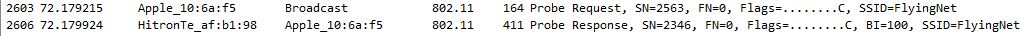
\includegraphics[scale = 0.6]{ex-11.JPG}
	\caption{Probing request e Probing response}
\end{figure}

\section{Processo de Associação}
\subsection{Ex12}
\textbf{Identifique uma sequência de tramas que corresponda a um processo de associação completo entre a STA e o AP, incluindo a fase de autenticação.}\\\par
Estas tramas podem ser encontradas usando o filtro wlan.fc.type\_subtype == 0 \textbar\textbar wlan.fc.type\_subtype == 1 \textbar\textbar wlan.fc.type\_subtype == 11, onde o primeiro campo corresponde a um pedido de associação, o segundo corresponde a uma resposta a um pedido de autenticação, e o ultimo corresponde à autenticação.

\begin{figure}[h]
	\centering
	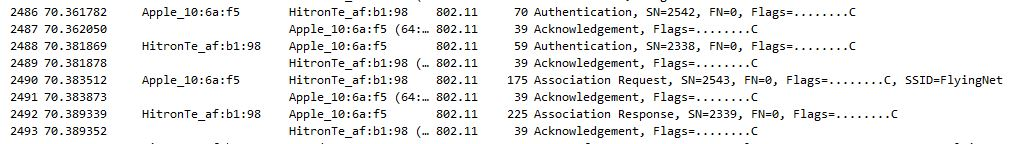
\includegraphics[scale = 0.6]{ex-12.JPG}
	\caption{Tramas do processo de associação}
\end{figure}

\newpage
\subsection{Ex13}
\textbf{Efetue um diagrama que ilustre a sequência de todas as tramas trocadas no processo.}\\\par

\begin{figure}[h]
	\centering
	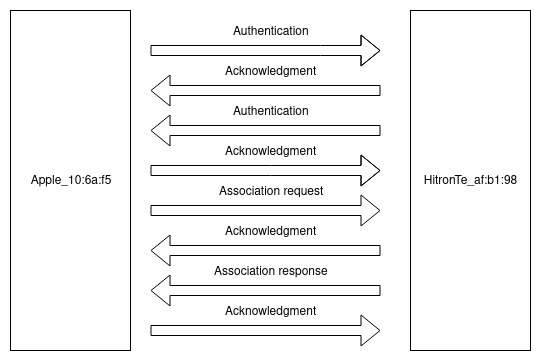
\includegraphics[scale = 0.6]{diagrama-ex13.jpeg}
	\caption{Tramas do processo de associação}
\end{figure}


\section{Transferência de Dados}
\subsection{Ex14}
\textbf{Considere a trama de dados nº455. Sabendo que o campo Frame Control contido no cabeçalho das tramas 802.11 permite especificar a direccionalidade das tramas, o que pode concluir face à direccionalidade dessa trama, será local à WLAN?}\\\par
Uma vez que o campo \texit{To DS} está a 0 e o \textit{From DS} está a 1, podemos concluir que a direcionalidade da trama foi da estação para o Sistema de Distribuição. Desta forma, como o destino da trama é exterior ao BSS, podemos concluir que a direcionalidade da trama não é local à WLAN. 
\begin{figure}[h]
	\centering
	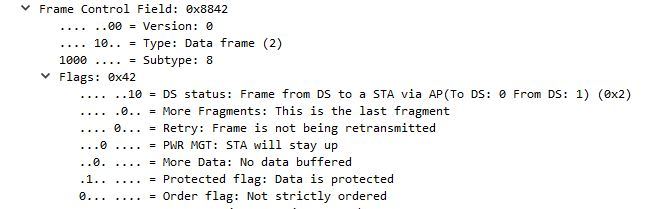
\includegraphics[scale = 0.6]{ex-14.JPG}
	\caption{Flags da trama 455}
\end{figure}

\subsection{Ex15}
\textbf{Para a trama de dados nº455, transcreva os endereços MAC em uso, identificando qual o endereço MAC correspondente ao host sem fios (STA), ao AP e ao router de acesso ao sistema de distribuição?}\\\par
O endereço MAC correspondete ao host sem fios (STA) é d8:a2:5e:71:41:a1, já o do AP é d8:a2:5e:71:41:a1, e por fim, o endereço MAC do router de acesso ao sistema de distribuição é bc:14:01:af:b1:98.
\begin{figure}[h]
	\centering
	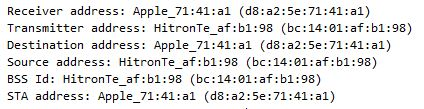
\includegraphics[scale = 0.6]{ex-15.JPG}
	\caption{Endereços MAC}
\end{figure}

\subsection{Ex16}
\textbf{Como interpreta a trama nº457 face à sua direccionalidade e endereçamento MAC?}\\\par
Uma vez que o campo \texit{To DS} está a 1 e o \textit{From DS} está a 0, podemos concluir que a direcionalidade da trama foi do Sistema de Distribuição para a estação. Além disso, podemos concluir que 
\begin{figure}[h]
	\centering
	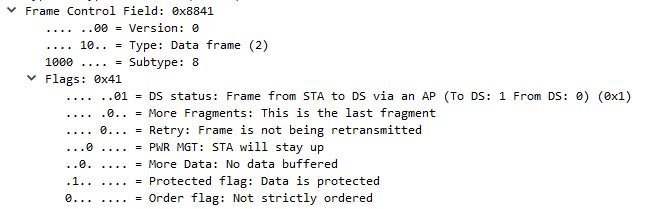
\includegraphics[scale = 0.6]{ex-16.JPG}
	\caption{Flags da trama 457}
\end{figure}

\subsection{Ex17}
\textbf{Que subtipo de tramas de controlo são transmitidas ao longo da transferência de dados acima mencionada? Tente explicar porque razão têm de existir (contrariamente ao que acontece numa rede Ethernet.)}\\\par
Ao longo da transferência de dados, são transmitidas tramas de controlo de erros denominadas acknowlegments. Estas tramas são fundamentais nas redes sem fios, uma vez que nestas a probabilidade de ocorrencia de erros é muito superior à de uma rede ethernet, por exemplo, não estando implementado nenhum método de controlo de erros. Para contornar este problema, as estações enviam sempre um acknowledgment para comunicar ao emissor que a mensagem foi bem recevida, o que permite determinar se ocorreram erros na transferencia de dados.

\subsection{Ex18}
\textbf{O uso de tramas Request To Send e Clear To Send, apesar de opcional, é comum para efetuar "pré-reserva" do acesso ao meio quando se pretende enviar tramas de dados, com o intuito de reduzir o número de colisões resultante maioritariamente de STAs escondidas. Para o exemplo acima, verifique se está a ser usada a opção RTS/CTS na troca de dados entre a STA e o AP/Router da WLAN, identificando a direccionalidade das tramas e os sistemas envolvidos.}\\\par
Como podemos observar na imagem, as tramas RTS (\textit{Request To Send}) e CTS (\textit{Clear To Send}) estão a ser utilizadas na troca de dados entre o AP e o STA, sendo a trama 533 um RTS e a trama 534 um CTS. Neste caso, o STA corresponde ao Apple\_10:6a:f5 e o AP ao HitreonTe\_af:b1:98. Além disso, como as flags \textit{To DS} e \textit{From DS} estão ambas a zero, podemos concluir que a direcionalidade da trama é local à WLAN.
\newpage
\begin{figure}[h]
	\centering
	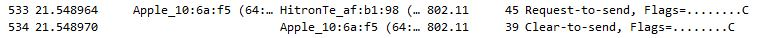
\includegraphics[scale = 0.6]{ex-18.JPG}
	\caption{Tramas RTS e CTL}
\end{figure}

\begin{figure}[h]
	\centering
	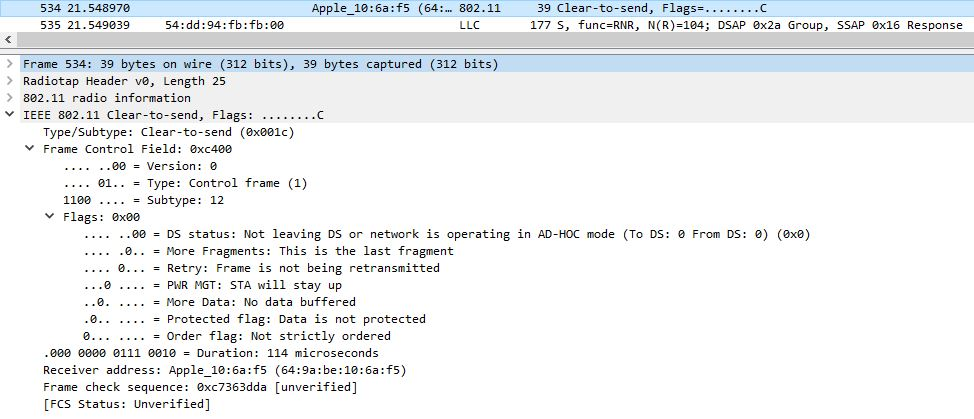
\includegraphics[scale = 0.5]{ex-18-trama534.JPG}
	\caption{Trama 534}
\end{figure}

\begin{figure}[h]
	\centering
	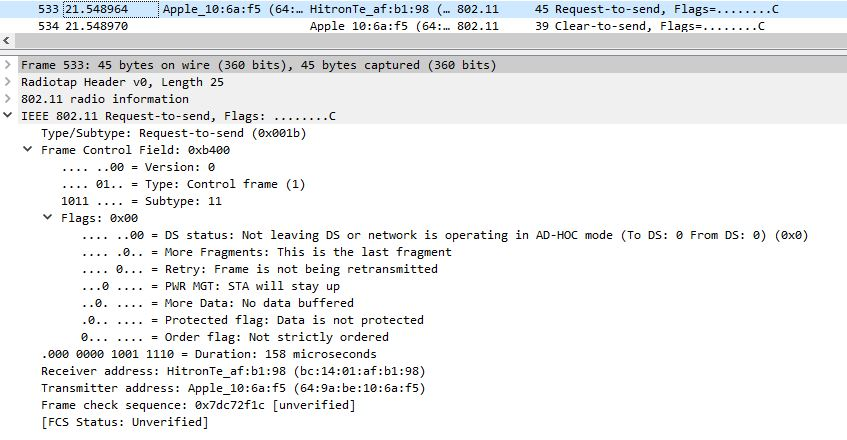
\includegraphics[scale = 0.5]{ex-18-trama533.JPG}
	\caption{Trama 533}
\end{figure}

\section{Conclusão}
Este trabalho prático serviu de complemento às aulas teóricas e ajudou a consolidar a matéria lecionada nas mesmas.\par
Depois de finalizado o trabalho prático, relativo às Redes Wireless, obtivemos mais conhecimentos sobre o funcionamento ao nível da rede das redes wi-fi.
Conceitos como, tipos e subtipos de tramas, STA, AP e direcionalidade de tramas foram recordados e aplicados. Além disso investimos mais tempo a compreender quais o funcionamento dos filtros no WireShark para encontrar diversas tramas, o que se revelou uma mais valia tendo em conta as perguntas onde foram úteis.\par
Desta forma, consideramos que os objetivos pretendidos pelo trabalho foram compridos.
\end{document}
